\clearpage
\sffamily
{\bfseries\color[rgb]{0.4,0.4,0.4}
Law 4 -- The Players ('Equipment')}
\phantomsection
\addcontentsline{toc}{section}{Law 4 -- The Players ('Equipment')}

\bigskip

{\bfseries Safety }

\headlinebox

A player must not use equipment or wear anything that is dangerous to himself or another player (including any kind of jewellery).

\bigskip

{\bfseries The Design of the Robots (new)}

\headlinebox

Robots participating in the Humanoid League competitions must have a human-like body plan, as shown in Fig. \ref{fig:bodyplan}. They must consist of two legs, two arms, and one head, which are attached to a trunk.

\bigskip

(new:) Robots in kid and teen size sub-leagues must be equipped with a handle, to be picked up safely and with no harm to the robot and the handler.

\begin{center}
\begin{figure}[h]
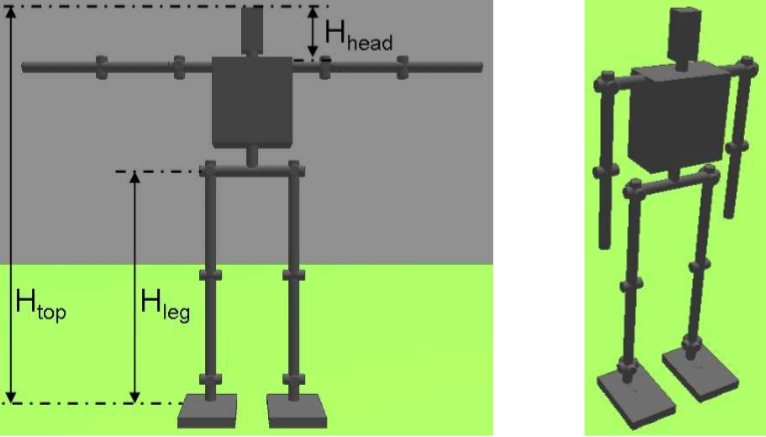
\includegraphics[width=\textwidth]{img/bodyplan.png}
\caption{Example of a humanoid robot body plan (left) and standing upright pose (right)}
\label{fig:bodyplan}
\vspace{-3ex}
\end{figure}
\end{center}

The robots must be able to stand upright on their feet and to walk on their legs. KidSize and TeenSize robots need to be able to recover from a fall (get back to a standing position). The only allowed modes of locomotion are bipedal walking, running and jumping.

\bigskip

All actions of the robots must be kinematically equivalent to humanoid motions.

\bigskip

{\bfseries Robot Height (new)}

\headlinebox

Based on $H_{top}$, the following size restrictions apply:

\begin{itemize}
\item 40cm ${\leq}$ $H_{top}$ ${\leq}$ 90cm to play in the KidSize class, 
\item 80cm ${\leq}$ $H_{top}$ ${\leq}$ 140cm to play in the TeenSize class,
\item 130cm ${\leq}$ $H_{top}$ ${\leq}$ 180cm to play in the AdultSize class.
\end{itemize}

$H_{top}$ is defined as the height of the robot when standing upright (with fully extended knees, cf. Fig. \ref{fig:bodyplan} right) and $H_{COM}$ denotes the height of the robot's center of mass, measured in upright posture. \added{$H_{top}$ is measured with the head of the robot oriented in such a way that it is tilted to either its maximum upwards tilt angle or the horizon line, whichever is lower.}

\bigskip

{\bfseries Weight Restrictions (new)}

\headlinebox
\begin{itemize}
\item The maximum weight for robots allowed to play in the TeenSize class is 20 kg.
\item The minimum weight for robots allowed to play in the AdultSize class is 10 kg
\end{itemize}

\bigskip

{\bfseries Size Restrictions (new)}

\headlinebox

All robots participating in the Humanoid League must comply with the following restrictions:

\begin{itemize}
\item Each foot must fit into a rectangle of area $\tfrac{1}{32} (2.2 \cdot H_{COM})^2$. 
\item Considering the rectangle enclosing the convex hull of the foot, the ratio between the longest side of the rectangle and the shortest one, shall not exceed $2.5$.
\item The robot must fit into a cylinder of diameter $0.55 \cdot H_{top}$.
\item The robot does not possess a configuration where it is extended longer than 1.5{\textperiodcentered}$H_{top}$ .
\item The length of the legs $H_{leg}$, including the feet, satisfies 0.35{\textperiodcentered}$H_{top}$ ${\leq}$ $H_{leg}$ ${\leq}$ 0.7{\textperiodcentered}$H_{top}$ .
\item The height of the head $H_{head}$, including the neck, satisfies $0.05 \cdot H_{top} \leq H_{head} \leq 0.25 \cdot H_{top}$. $H_{head}$ is defined as the vertical distance from the axis of the first arm joint at the shoulder to the top of the head. 
\item The leg length is measured while the robot is standing up straight. The length is measured from the first rotating joint where its axis lies in the plane parallel to the standing ground to the tip of the foot.
\item The minimum length of the arm, measured from the first joint, is $H_{top} - H_{leg} - H_{head}$.
\end{itemize}


{\bfseries Sensors (new)}

\headlinebox

Teams participating in the Humanoid League competitions are encouraged to equip their robots with sensors that have an equivalent in human senses. These sensors must be placed at a position roughly equivalent to the location of the human{\textquoteright}s biological sensors. In particular, 

\begin{itemize}
\item The only active external sensor allowed is sound
(``human-like'' with respect to volume and frequency) with one loudspeaker on the robot. The loudspeaker may be placed in the head, neck or trunk of the robot. Any
other active sensor (emitting light, sound, or electromagnetic waves into the environment in order to measure reflections) is not allowed. 
\item External sensors, such as cameras and up to two microphones, may not be placed in the legs or arms or the
torso of the robots. They must be placed in the robot's
head and above any neck joint. 
\item The number of cameras is limited to a stereo vision setup (i.e., max. 2 cameras with a large overlap) only. Monocular vision is also allowed.
\item The field of view of the robots is limited at any time to $180$ degrees. This means that the maximum angle between any two points in the union of the field of view of all cameras mounted on the robot must be less than $180$ degrees. Also the pan-tilt motion of the head and the cameras mounted on the robot's head is restricted to be more human like not only with respect to the field of view but also to the range of motion of the neck joints. Therefore, the mechanism to pan the camera is limited to $270$ degree pan, which means $\pm135$ degrees from the position looking straight ahead. The mechanism to tilt the camera is limited to $\pm90$ degrees (measured from the horizontal line). Furthermore, if positioned at the center mark the robot may not be able to see \added{more than two goal posts} \removed{both goals} in any tilt angle and in any standing or walking posture of the robot. 
\item Touch sensors, force sensors, and temperature sensors may be placed at any position on the robot.
\item Sensors inside the robot may measure all quantities representing the local state of the system, including (but not limited to) voltages, currents, forces, movements, accelerations, and rotational speeds. They can be at any position inside the robot. Measurements from earth magnetic field sensors may not be used in the software and - in case of doubt - the code must be made available to members of the Technical Committee for inspection.
\end{itemize}

{\bfseries Communication and Control (new)}

\headlinebox

Robots participating in the Humanoid League competitions must act autonomously while a competition is running. No external power supply, teleoperation, remote control, or remote brain of any kind is allowed.

\bigskip

Robots may communicate only via the wireless network provided by the organizers, which must support the referee box. The total bandwidth of the robots belonging to one team may not exceed 1 Mbit/s. The robots must not rely on the quality of the wireless network. They
must be able to play if the network is of low quality. Only robots are allowed to communicate by WLAN. Any other computers of team members are only allowed to communicate by tethered LAN. No other wireless communication is allowed onsite. All other wireless hardware must be deactivated. A team may be disqualified if one of the team members violates this rule.

\bigskip

Robots in play may communicate with each other at any time during a game. Any kind of transmission from an external computer or an out of play robot to the playing robots is prohibited. This implies that any monitoring is only done by receiving UDP communication from the robots using an external computer connected by tethered LAN to the official wireless router. 

\bigskip

Sending any direct or indirect transmission from an external computer to the robots has to take place during a timeout or service of the robot. Connecting a LAN cable to the robot is automatically considered service. Any other type of communication with the robot, excluding verbal communication of the robot handler and pressing a button to start or stop the robot's general behaviour, has to be announced to the referee so a service penalty can be given to the respective robot. If the team does not announce the communication before starting it, an additional 30 second penalty is given to the team. In case of repeated violation, the referee may take disciplinary actions against the team as defined in Law 5.
\bigskip

Teams may not use any type of communication, excluding verbal communication, with robots in play, in service or with robots suffering a removal penalty that contains information which reduces the need for autonomy in detecting the current game state of the robots, including the position of the ball, the location where the robot re-enters the field, the orientation of the robots own or opponents goal, and the position of team members or opponents. In case of doubt that a team violates this rule, the code must be made available to members of the Technical Committee for inspection.

\bigskip

During the game an official game controller/referee box will be used. It uses UDP to broadcast information to the robots like elapsed time, current score, game state (ready, set, playing, finished) and the robot-specific penalized state. The source code is open. To encourage teams to use the referee box, 15 seconds advantage is given to teams using the referee box in any stoppage of the game.



\bigskip

In KidSize and TeenSize, no humans are allowed on the field while the ball is in play. Robot handlers stay in a designated area and must receive permission from the referee prior to entering the field. Each team may designate only one person as robot handler. The robot handler of a team may not touch a robot of another team in order to avoid any (unintentional or intentional) damage to that robot. 

\bigskip

The source code of the game controller/referee box is available from

\textcolor[rgb]{0.0,0.0,0.49803922}{https://github.com/RoboCup-Humanoid-TC/GameController},
see also 

\textcolor[rgb]{0.0,0.0,0.49803922}{https://www.robocuphumanoid.org}.

\simplify{
\bigskip

\greyed{
{\bfseries (suspended: Basic equipment}

\headlinebox

The basic compulsory equipment of a player comprises the following separate items:

\begin{itemize}
\item a jersey or shirt with sleeves -- if undergarments are worn, the colour of the sleeve must be the same main colour as the sleeve of the jersey or shirt 
\item shorts -- if undershorts or tights are worn, they must be of the same main colour as the shorts
\item stockings -- if tape or similar material is applied externally it must be the same colour as that part of the stocking it is applied to shinguards footwear) 
\end{itemize}
}

\bigskip

\greyed{
{\bfseries (suspended: Shinguards}

\headlinebox

\begin{itemize}
\item are covered entirely by the stockings
\item are made of rubber, plastic or a similar suitable material 
\item provide a reasonable degree of protection)
\end{itemize}
}
}

\bigskip

{\bfseries Colours}

\headlinebox

\begin{itemize}
\item (new) Robots must be mostly black or of dark grey color (i.e. RAL 7011 Iron Grey or darker) and non reflective. Robots may also be colored in aluminimum-like silver, grey or white but then their feet must be colored black. Any color used for the field (green, white) or colors similar to the opponent team's team markers must be avoided. Arms, legs and bodies of the robot must be of solid shape appearance.
\item (new) The robots must be marked with team markers. These markers are colored \removed{magenta (referred to as red)} \added{red} for one team and \removed{cyan (referred to as blue)} \added{blue} for the other team. Robot legs and arms must be covered by team markers. From each side of the robot, at least one team marker must be visible on both an arm and a leg. The marker must cover an area of at least \added{$0.15\cdot H_{top}$ x $0.05\cdot H_{top}$} \removed{be at least 5 cm in height and as wide as the leg or arm of the robot as seen from that side}. If both teams cannot agree, which team color to use, a coin will be flipped \added{an hour} \removed{15 minutes} prior to the game to assign the team colors.
\item (new) The robots of each team must be uniquely identifiable. They must be marked with numbers or names. The goal keeper robot must be marked uniquely that it can be easily distinguished from the other robots of a team by the referees. 
\item The two teams must wear colours that distinguish them from each other and also the referee and the assistant referees.
\greyed{\item 
(suspended: Each goalkeeper must wear colours that distinguish him from the other players, the referee and the assistant referees) }
\end{itemize}

\bigskip

{\bfseries Infringements and sanctions}

\headlinebox

In the event of any infringement of this Law:

\begin{itemize}
\item play need not be stopped
\item the player at fault is instructed by the referee to leave the field of play to correct his equipment
\item the player leaves the field of play when the ball next ceases to be in play, unless he has already corrected his equipment
\item any player required to leave the field of play to correct his equipment must not re-enter without the referee's permission
\item the referee checks that the player's equipment is correct before allowing him to re-enter the field of play 
\item the player is only allowed to re-enter the field of play before the respective penalty time is over \greyed{ (replaces: when the ball is out of play)}
\end{itemize}

\bigskip

A player who has been required to leave the field of play because of an infringement of this Law and who re-enters the field of play without the referee's permission must be cautioned.

\bigskip

\clearpage
{\bfseries Restart of play}

\headlinebox

If play is stopped by the referee to administer a caution:

\begin{itemize}
\item the match is restarted by an indirect free kick taken by a player of the opposing team from the place where the ball was located when the referee stopped the match (see Law 13 -- Position of free kick)
\end{itemize}

\bigskip


{\bfseries Decisions of the International F.A. Board }

\headlinebox

Decision 1

Players must not reveal undergarments showing slogans or advertising. The basic compulsory equipment must not have any political, religious or personal statements. A player removing his jersey or shirt to reveal slogans or advertising will be sanctioned by the competition organiser. The team of a player whose basic compulsory equipment has political, religious or personal slogans or statements will be sanctioned by the competition organiser (new) or by RoboCup Federation Humanoid League.
